\chapter{Benutzerverwaltung}
In einem ASP.NET MVC 4 Projekt ist bereits eine vollst�ndige Benutzerverwaltung integriert,
die wir auch in unserem Projekt benutzen wollen. Durch die integrierte Benutzerverwaltung 
sind Webseiten zur Registrierung und f�r den Login / Logout bereits fertig. 

\begin{figure}[H]
\centering
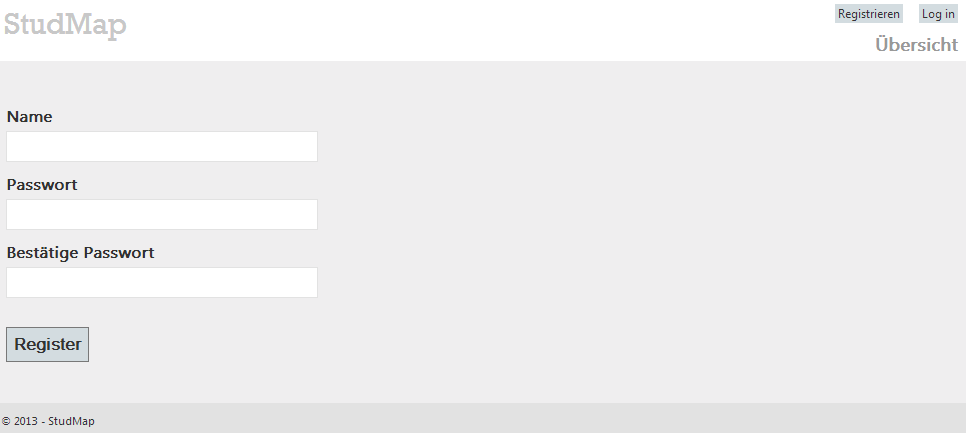
\includegraphics[width=0.7\linewidth]{../Bilder/RegisterSite}
\caption{Webseite zur Registrierung im StudMap Admin}
\label{fig:RegisterSite}
\end{figure}

F�r die Benutzerverwaltung verwendet das ASP.NET MVC 4 Projekt folgende Datenbankstruktur:
\begin{figure}[H]
\centering
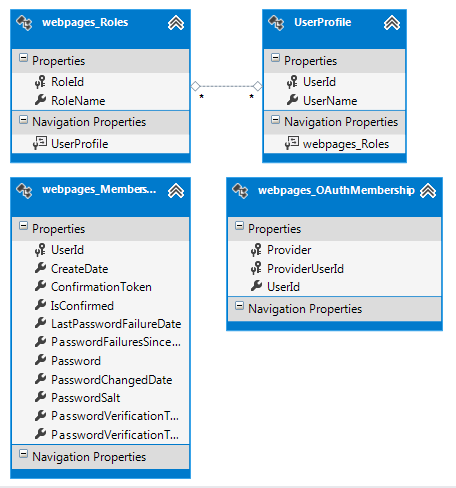
\includegraphics[width=0.7\linewidth]{../Bilder/GeneratedUserEntities}
\caption{Datenbankstruktur der integrierten Benutzerverwaltung}
\label{fig:GeneratedUserEntities}
\end{figure}

F�r unser Projekt sind nur die drei Tabellen \texttt{UserProfile}, \texttt{webpages\_Roles} und \texttt{webpages\_Membership} relevant. Wie im Domain Model bereits beschrieben unterscheiden wir zwischen den Benutzerrollen Benutzer und Administrator. Jeder Anwender kann sich in mehreren Benutzerrollen befinden. Zus�tzlich sind in der Tabelle \texttt{webpages\_membership} weitere Anwenderdaten wie beispielsweise das Datum der Registrierung das Passwort hinterlegt. Damit ist die Benutzerverwaltung f�r den Administrationsbereich vollst�ndig.


Um die am System angemeldeten Clients zu verwalten haben wir eine weitere Tabelle \texttt{ActiveUsers} hinzugef�gt:

\begin{figure}[H]
\centering
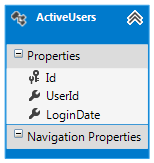
\includegraphics[width=0.7\linewidth]{../Bilder/ActiveUsersEntity}
\caption{Tabelle ActiveUsers}
\label{fig:ActiveUsersEntity}
\end{figure}

In dieser Tabelle werden Anwender gespeichert, die gerade aktiv mit dem Smartphone angemeldet sind.



\section{Service Schnittstelle}
F�r den StudMap Admin gen�gt die bereits integrierte Benutzerverwaltung. Allerdings ben�tigen wir noch eine Schnittstelle, damit auch die Web bzw. Smartphone Clients auf die Benutzerverwaltung zugreifen k�nnen.

Dazu gibt es im StudMap.Service Projekt einen \texttt{UsersController} der folgende Funktionen bereitstellt:


\begin{itemize}
\item Register
\item Login
\item Logout
\item GetActiveUsers
\end{itemize}


\subsection{Register}
Registriert einen neuen Anwender in der Benutzerrolle \textit{Benutzer}.

Aufruf �ber HTTP Post:\\
\url{http://localhost:1129/api/Users/Register?userName=test&password=geheim}


\subsection{Login}
Meldet einen bereits registrierten Anwender am System an.

Aufruf �ber HTTP Post:\\
\url{http://localhost:1129/api/Users/Login?userName=test&password=geheim}

\subsection{Logout}
Meldet einen angemeldeten Anwender vom System ab.

Aufruf �ber HTTP Get:\\
\url{http://localhost:1129/api/Users/Logout?userName=test}

\subsection{GetActiveUsers}
Ermittelt eine Liste der aktuell am System angemeldeten Anwender.

Aufruf �ber HTTP Get:\\
\url{http://localhost:1129/api/Users/GetActiveUsers}
